Ниже приведены графики, полученные в результате работы реализованной программы.

\begin{figure}[H]
	\begin{center}
		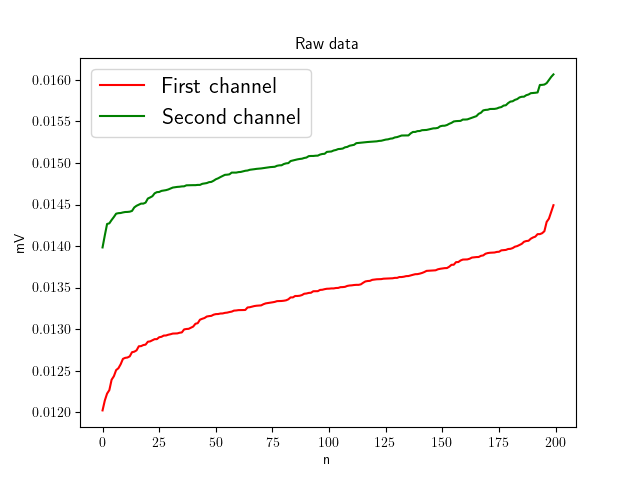
\includegraphics[scale=1]{rawdata}
		\label{pic:rawdata}
		\caption{Загруженные данные}
	\end{center}
\end{figure}

\begin{figure}[H]
	\begin{center}
		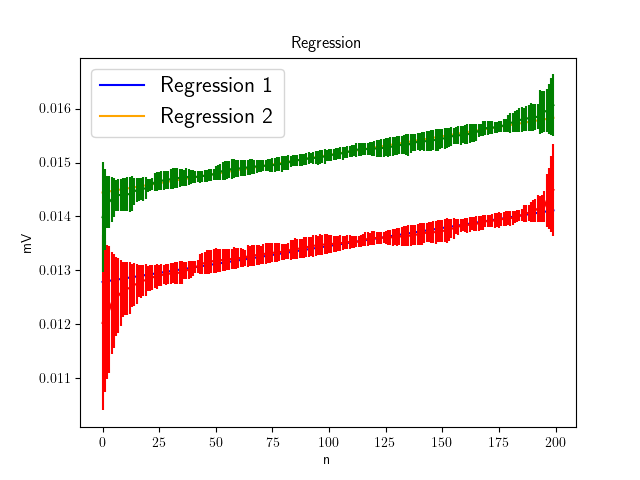
\includegraphics[scale=0.35]{regression}
		\label{pic:regression}
		\caption{Линейная регрессия для вещественных данных и результаты обынтерваливания}
	\end{center}
\end{figure}

\begin{figure}[H]
	\begin{center}
		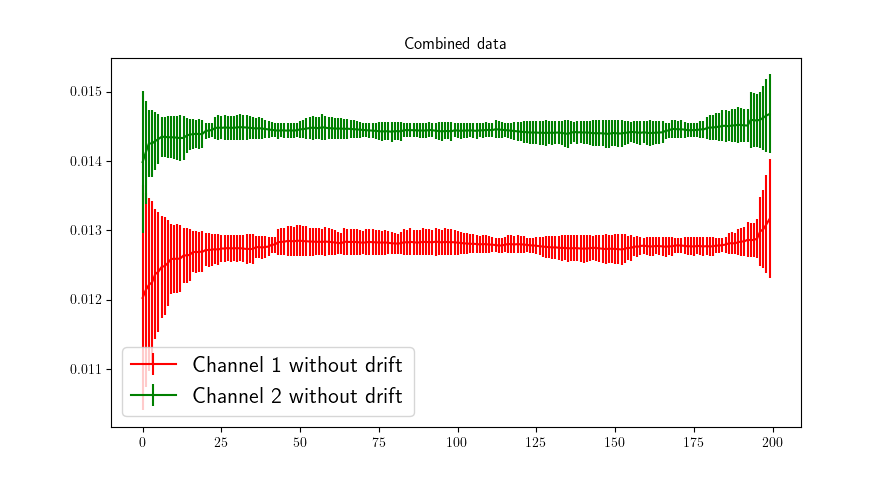
\includegraphics[scale=0.35]{horizontal}
		\label{pic:horizontal}
		\caption{Данные после вычитания ``наклонной'' составляющей}
	\end{center}
\end{figure}

\begin{figure}[H]
	\begin{center}
		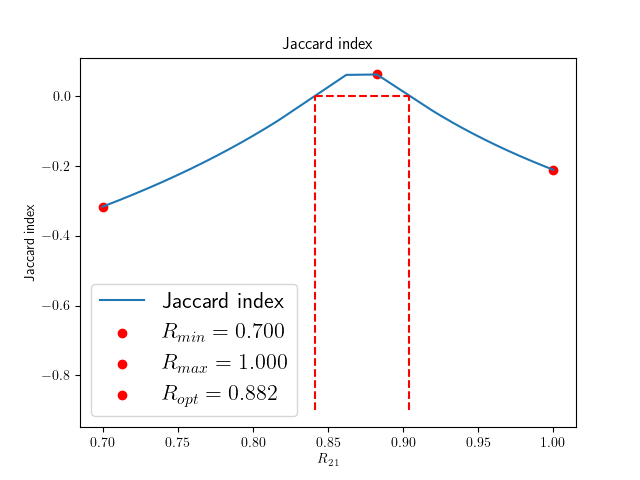
\includegraphics[scale=0.95]{jaccard}
		\label{pic:jaccard}
		\caption{Зависимость коэффициента Жаккара от $R_{21}$}
	\end{center}
\end{figure}

\begin{figure}[H]
	\begin{center}
		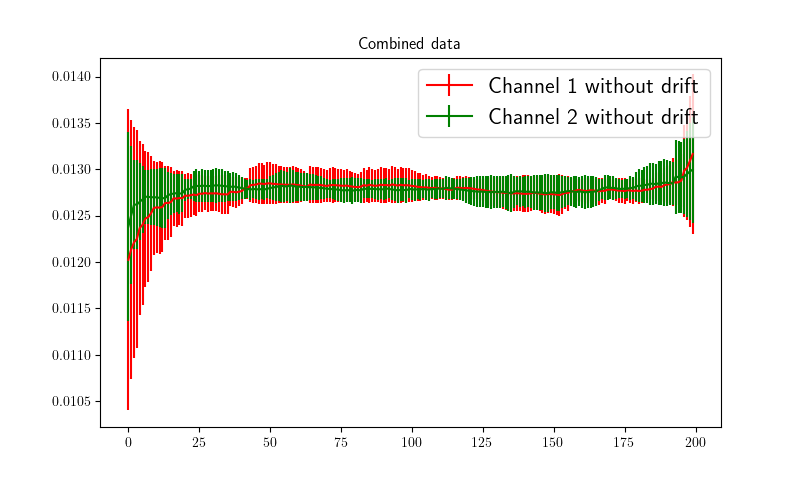
\includegraphics[scale=0.35]{result}
		\label{pic:result}
		\caption{Результат наложения данных при максимальном коэффициенте Жаккарда}
	\end{center}
\end{figure}